\documentclass{article}
\usepackage[utf8]{inputenc}
\usepackage{amsmath, amsfonts}
\usepackage{bm}
\usepackage{enumitem}
\usepackage{graphicx}
\usepackage[procnames]{listings}
\usepackage{color}
\usepackage{hyperref}



\usepackage{verbatim}
\usepackage{algorithm}
\usepackage{algpseudocode}

\usepackage{lingmacros}
\usepackage{tree-dvips}

\usepackage{verbatim}
\usepackage{algorithm}
\usepackage{algpseudocode}

\usepackage{tabu}

\usepackage{lingmacros}
\usepackage{tree-dvips}
\usepackage{ifthen}
\usepackage{mdwlist}
\DeclareMathOperator{\argmax}{argmax}
\newcommand{\argmin}{\operatornamewithlimits{argmin}}


\newtheorem{theorem}{Theorem}
\newtheorem{question}{Question}
\newtheorem{observation}{Observation}
\newtheorem{fact}[theorem]{Fact}
\newtheorem{lemma}[theorem]{Lemma}
\newtheorem{claim}{Claim}
\newtheorem{dfn}{Definition}
\newtheorem{definition}{Definition}
\newtheorem{corollary}{Corollary}
%\newtheorem{question}{Question}
\newcommand{\proofstart}{{\bf Proof\hspace{2em}}}
\newcommand{\tset}{\mbox{$\cal T$}}
\newcommand{\proofend}{\hspace*{\fill}\mbox{$\Box$}}
\newcommand{\bfm}[1]{\mbox{\boldmath $#1$}}



\title{EE227BT Project:
Understanding the Continuous-Time Limit of Nesterov Acceleration}
\author{Nilesh Tripuraneni (nilesh\_tripuraneni@berkeley.edu, 3032089919)\\ Sarah Dean (sarahdean@eecs.berkeley.edu, 3031893242)\\ Jeffrey Chan (chanjed@berkeley.edu, 24988067)\\ Aldo Pacchiano (pacchiano@berkeley.edu, 26995108)}



\begin{document}


\maketitle 

\section{Background}

Many convex optimization methods can be interpreted as the discretization of an ordinary differential equation -- whose solution trajectories approximate the steps of the optimization algorithm. The established theory of ordinary differential equations and dynamical systems can often provide insight in the design and analysis of their corresponding discrete-time optimization algorithms. Connections between these fields have been fruitfully explored in the classical optimization literature in a number of works \cite{helmke2012optimization, schropp2000dynamical, fiori2005quasi, durr2012class, dorr2012smooth, osher2016sparse, qin2012structured, lessard2016analysis}.

In the present work we both review and advance the connection between first-order gradient methods for optimization and their continuous-time counterparts -- in particular focusing on the continuous-time limit of Nesterov's accelerated gradient method. First-order methods have regained popularity in machine learning and many other fields as data sets and problems increase in size and complexity. Thirty years ago, however, in a seminal paper Nesterov proposed a family of ``accelerated" gradient algorithm provably improving upon the convergence rate of ordinary gradient descent \cite{nesterov1983method} \footnote{Nesterov proposed two distince schemes for both accelerating gradient descent applied to both weakly and strongly convex functions -- we henceforth refer to Nesterov (I) for the scheme for weakly convex functions and Nesterov (II) for the scheme for strongly convex functions}. While these ``accelerated" methods are easy to implement, the convergence proofs of these ``accelerated" first-order gradient schemes have long been considered difficult to understand. Further, many researchers have also lacked an intuitive understanding of ``why" these methods work -- making them difficult to generalize as well.

A recent line of research initiated by \cite{su2014differential} derived, perhaps surprisingly, a \textit{second-order} ODE which is the exact limit of the \texit{first-order} Nesterov (I) scheme. Various examples and case studies related to this second-order ODE provided in \cite{su2014differential} used this conceptually simpler ODE as a tool for understanding, analyzing and generalizing Nesterov’s scheme. Since then, several researchers have attempted to both extend this work into more general settings and further understand the significance of the discretization between the continuous-time ODE perspective and the original discrete-time Nesterov schemes \cite{krichene2015accelerated, wibisono2016variational, wilson2016lyapunov}.

The purpose, structure, and contributions of this project can be broadly summarized as:
\begin{itemize}
    \item Reviewing accelerated first-order methods in both discrete and continuous time focusing on establishing the optimality lower bounds shown in \cite{nesterov2004introductory} and introducing the second-order scheme analyzed in \cite{su2014differential} for the Nesterov (I) scheme.
    \item Extending results of \cite{su2014differential} to the case of the Nesterov (II) scheme which is applicable to strongly convex functions. This includes producing both continuous-time convergence proofs for gradient descent and the Nesterov (II) scheme we derive and providing intuitive perspective connecting the Nesterov (II) scheme to the physics of the damped harmonic oscillator.
    \item Investigating the generalization of the Nesterov (I) scheme to non-Euclidean geometries -- i.e. ``accelerated" mirror descent -- studied in \cite{krichene2015accelerated}.
\end{itemize}

\subsection{Gradient Descent}

Gradient descent is an iterative optimization algorithm that can be used to minimize a function $f$ over $\mathbb{R}^{d}$. The iterates evolve as:
\begin{equation}
    x_{k+1} = x_k - s \nabla f(x_k)
\end{equation}
where $s > 0$ is the step size. 

One can provably show the convergence of gradient descent algorithm when it is used to minimize a \textit{convex} function subject to smoothness conditions on the function $f$. In particular, depending on the type of convex function we can derive different rates of convergence for its quickness in finding the global optima of $f(x)$, $x^*$. 

\begin{figure}[!h]
\begin{center}
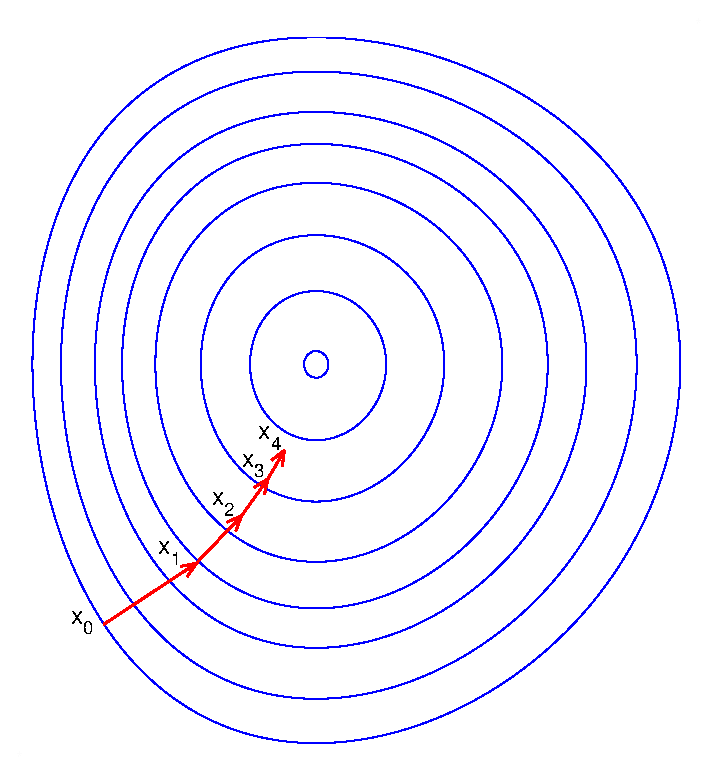
\includegraphics[width=0.2\linewidth]{SourceFiles/plots/Gradient_descent.eps}
\caption{Gradient Descent iterates moving towards the global optimum.}
\end{center}
\end{figure}

To this end, it is interesting to consider the class of functions which are restricted to being $\beta-$smooth and $\alpha-$strongly convex. 
We now recall these definitions:
\begin{definition}
If $f$ is a differentiable, convex function and $x,y$ two points in its domain, then:
\begin{equation}\label{convexity_def_eq}
f(y) \geq f(x) + \nabla f'(x)^\top (y-x)
\end{equation}
\end{definition}

\begin{definition}
$f$ is $\alpha-$strongly convex if:
\begin{equation}
f(y) \geq f(x) + \nabla f(x)^\top(y-x) + \frac{\alpha}{2} ||x - y||_2^2
\end{equation}
\end{definition}

Alternatively, a function $f$ is strongly convex if $x \rightarrow f(x) - \frac{\alpha}{2} ||x||^2$ is convex. In the case of twice differentiable functions this is equivalent to $\nabla^{2} f(x) \succeq \alpha I$. Intuitively, this is equivalent to stating that $f$ is globally \textit{lower-bounded} by a quadratic function. 

\begin{definition}
$f$ is $\beta$-smooth if:
\begin{equation}\label{fundamental_beta_eq}
f(y) \leq f(x) + \nabla f(x)^\top(y-x)+ \frac{\beta}{2} ||x - y||_2^2
\end{equation}
\end{definition}
Alternatively, a function $f(x)$ is $\beta$-smooth if its gradients $\nabla f(x)$ are $\beta-$Lipschitz:
\begin{equation}
    || \nabla f(x) - \nabla f(y) || \leq \beta ||x - y||
\end{equation}
In the case of twice differentiable functions this is equivalent to $\nabla^{2} f(x) \preceq \beta I$.
Intuitively, this is equivalent to stating that $f$ is globally \textit{upper-bounded} by a quadratic function.

If $f$ is $\alpha-$ strongly convex and $\beta-$ smooth then:
\begin{definition}
The \textbf{condition number} of $f$ is $\kappa = \frac{\beta}{\alpha}$. 
\end{definition}

\subsection{Convergence Rates}

It is well-known that gradient descent applied to a $\beta-$smooth functions achieves a $\mathcal{O}(1/k)$ convergence rate \cite{DBLP:journals/ftml/Bubeck15}:

\begin{theorem}
Let $f$ be convex and $\beta$-smooth then gradient descent with $s = \frac{1}{\beta}$ satisfies:
\begin{equation}
f(x_k) - f(x^*) \leq \frac{2\beta ||x_1 - x^* ||_2^2}{k-1}
\end{equation}
\end{theorem}

The proof of this result hinges on the use of equations \ref{fundamental_beta_eq}, \ref{convexity_def_eq} which immediately imply a bound for the minimal improvement of a single gradient descent step: $
f(x- \frac{1}{\beta} \nabla f(x) ) - f(x) \leq -\frac{1}{2\beta} ||\nabla f(x)||^2$

If the function $f$ is smooth and strongly convex the convergence rate of gradient descent is improved from $\mathcal{O}(1/t)$ to $\mathcal{O}(\exp(-t/\kappa))$ \cite{DBLP:journals/ftml/Bubeck15}:

\begin{theorem}
If $f$ is $\alpha-$strongly convex and and $\beta-$smooth then gradient descent with step size $s = \frac{2}{\alpha+\beta}$ satisfies:
\begin{equation}
f (x_{k+1}) - f(x^*) \leq \frac{\beta}{2} \exp(-\frac{4t}{\kappa+1}) ||x_1-x^*||_2^2
\end{equation}
\end{theorem}

As we will see in the next section these rates are not optimal. In fact, \cite{nesterov2004introductory} proved optimality lower bounds for the convergence rate of an first-order algorithm that can only access function and gradient evaluations. Remarkably, \cite{nesterov2004introductory} also presented an ``acceleration" scheme to achieve these lower bounds.

\begin{center}
 \begin{tabular}{||c c ||} 
 \hline
 Function Class  & Gradient Descent Convergence Rate \\ [0.5ex] 
 \hline\hline
 $\beta$-Smooth  & $\frac{1 }{k}$  \\ [1ex]
 \hline
 $\beta$-Smooth and $\alpha-$Strongly Convex   & $\exp\left(-\frac{k}{\kappa}\right)$  \\[1ex]
 \hline
\end{tabular}
\end{center}

\subsection{``Oracle" Lower bounds}

A black box optimization procedure is a mapping from the history of the algorithm to the next query point, in the algorithm's quest for the minimizer of $f$. A black-box, linear first-order optimization algorithm is any method such $x_1 = 0$ and produces the iterate $x_{k+1}$ from the values $(x_1, g_1, \cdots, x_k, g_k)$ such that $g_k \in \partial f(x_k)$ $x_{k+1} \in \text{span}(g_1, \cdots, g_k)$.  \cite{nesterov2004introductory} proved striking lower bounds showing that any black-box, linear first-order optimization algorithm could not descend a $\beta$-smooth convex function faster than at a  $\mathcal{O}(1/k^2)$ rate and a $\alpha$-strongly convex, $\beta$-smooth function faster than at a  $\mathcal{O}(\exp(-t/\sqrt{\kappa})$ rate.

In this section, we present proofs of these lower bounds for both classes of convex functions. Throughout this section we will use $e_1, \cdots, e_n$ to denote the canonical basis of $\mathbb{R}^n$, and $B_2(R) = \{ x \in \mathbb{R}^n : ||x|| \leq R\}$ the $\ell_2$-ball of radius $R$. We first show that for $\beta-$smooth convex functions there is no linear, first-order, black-box procedure achieving a faster convergence rate than $\mathcal{O}(\frac{1}{k^2})$. 

\begin{theorem}
Let $k \leq (n-1)/2 , \beta >0$, then there is a $\beta-$smooth convex function such that any black box procedure for which $x_{k+1} \in Span(g_1, \cdots, g_k)$: 

\begin{equation}
\min_{1 \leq a \leq t } f(x_a ) - f(x^*) \geq \frac{3\beta}{32} \frac{\parallel x_1 - x^*\parallel}{(k+1)^2}
\end{equation}

\end{theorem}




\proofstart


Consider the following quadratic function:

\begin{equation}
    f(x) = \frac{\beta}{8}x^T A_{2k+1}x- \frac{\beta}{4}x^Te_1
\end{equation}


Where $A_m$ is an $n\times n$ matrix defined as:

\begin{equation}
(A_m)_{i,j} = \begin{cases}
                2  &  i = i,j \leq k \\
                -1 &  j \in \{i-1, i+1\}, i \leq k, j \neq m+1\\
                0 & \text{o.w.}
            \end{cases}
\end{equation}

 
Define $f_m(x) = \frac{\beta}{8} x^T A_m x - \frac{\beta}{4}x^Te_1$ and for any function $g$ define $g^* = \min_{x \in \mathbb{R}} g(x)$.

The matrix $A_m$ satisfies the following additional properties:
\begin{itemize}
\item[1] $0 \preceq A_m \preceq 4I_n$
\item[2] $x^TA_mx = x(1)^2 + x(m)^2 + \sum_{i=1}^{m-1} (x(i)-x(i+1))^2$.
\item[3] If $y(i) = 0$ for $i \geq r$, then $y^T A_{2k+1} y = y^TA_{r}y$ and therefore by 2) $\nabla f(y) \in span(e_1, \cdots, e_{r})$. 
\item[4] The minimiser $x_m^*$ of $f_m(x)$ and its optimal value $f_m^*$ satisfy:
    \begin{align}
        x_m^*(i) = \begin{cases}
                    1-\frac{i}{m+1} & i = 1, \cdots, k \\
                    0 & \text{o.w.}
                    \end{cases}\\
        f_m^* = -\frac{\beta}{8}\left( 1-\frac{1}{m+1}\right)
    \end{align}
\end{itemize}


Notice that $x_m$ is in the span of $e_1, \cdots, e_{m-1}$.  Recall that $x_1 = 0$, and therefore that $\partial(f(x_1)) = -\frac{\beta}{4}e_1$, meaning that $x_2 \in span(e_1)$, by an inductive application of 3) we conclude that $x_m \in span(e_1, \cdots, e_{m-1})$. 

Combining the previous observations we conclude the following string of inequalities:


\begin{equation}
f(x_m) - f^* = f_s(x_m) - f_{2k+1}^* \geq f_m^* - f^*_{2k+1} \geq f_k^* - f_{2k+1}^*
\end{equation}

Since $\parallel x_m^* \parallel^2 = \sum_{i=1}^m \left( \frac{i}{m+1}\right)^2 \leq \frac{m+1}{3}$ we obtain:

\begin{equation}
f_k^* - f_{2k+1}^* =\frac{\beta}{8}\left( \frac{1}{k+1} - \frac{1}{2k+2}\right) \geq \frac{3\beta}{32} \frac{\parallel x_{2k+1}*\parallel^2}{(k+1)^2}
\end{equation}

This concludes the proof. 

\proofend









\begin{theorem}
If the condition number $\kappa > 1$, then there is a $\beta-$smooth and $\alpha-$strongly convex function $f: l_2 \rightarrow \mathbb{R}$ with $\kappa = \frac{\beta}{\alpha}$ such that for any $k \geq 1$ and any black box procedure for which $x_{m+1} \in Span( g_1, \cdots, g_m)$:

\begin{equation}
f(x_k) - f(x^*) \geq \frac{\alpha}{2} \left(\frac{ \sqrt{\kappa}-1}{\sqrt{\kappa}+1}\right)^{2(k-1)} \parallel x_1 - x^* \parallel^2
\end{equation}

When $\kappa$ is large, $\left(\frac{ \sqrt{\kappa}-1}{\sqrt{\kappa}+1}\right)^{2(t-1)} \parallel x_1 - x^* \parallel^2 \approx \exp( -\frac{4(t-1)}{\sqrt{\kappa}})$


\end{theorem}

\proofstart

The main ideas of this proof are very similar to those used in the previous one. Denote by $A$ the infinite dimensional linear operator corresponding to an inifinite matrix with $2$ in the diagonal, and $-1$ on the upper and lower diagonals. This operator is a generalization of the finite dimensional $A_m$ operators found in the previous section. 

We will show that the following $\alpha-$convex and $\beta-$smooth function:

\begin{equation}
f(x) = \frac{\alpha(\kappa-1)}{8} \left( \langle Ax, x \rangle - 2\langle e_1, x \rangle \right) + \frac{\alpha}{2} \parallel x \parallel^2
\end{equation}


Since $f$ is $\alpha-$strongly convex $f(x_m) - f(x^*) \geq \frac{\alpha}{2}\parallel x_m - x^*\parallel^2$. Therefore it only remains to lower bound $\parallel x_m - x^*\parallel^2$.

$A$ has similar properties to its finite version, namely $0 \preceq A \preceq 4I$ and $x_k(i) =0 \forall i \geq k$. The later immediately implies that: 

\begin{equation}
\parallel x_k - x^* \parallel^2 \geq \sum_{i=k}^\infty x^*(i)^2
\end{equation}

To instantiate the lower bound we compute $x^*$. After differentiating and setting the gradient to zero we find the optimum is achieved by $x^*$ satisfying:

\begin{equation}
x^*(i) = \left( \frac{\sqrt{\kappa} - 1}{\sqrt{\kappa} +1} \right)^i 
\end{equation}

Putting all these bound together:

\begin{equation}
f(x_k) - f(x^*) \geq \frac{\alpha}{2}\sum_{i=k}^\infty \left( \frac{\sqrt{\kappa} - 1}{\sqrt{\kappa} +1} \right)^{2i} 
\end{equation}

Recall that $x_1 =0$. The geometric sum can be rewritten as 
\begin{equation}
\left( \frac{\sqrt{\kappa} - 1}{\sqrt{\kappa} +1} \right)^{2(k-1)} \left( \sum_{i=1}^\infty \left( \frac{\sqrt{\kappa} - 1}{\sqrt{\kappa} +1} \right)^{2i} \right) = \left( \frac{\sqrt{\kappa} - 1}{\sqrt{\kappa} +1} \right)^{2(k-1)} \parallel x_1 - x^* \parallel^2
\end{equation}

This concludes the proof.

\proofend

The following table sumarizes the lower bounds above and the gradient descent rates. 

\begin{center}


 \begin{tabular}{||c c c ||} 
 \hline
 Function Class   & GD  & Lower bound \\ [0.5ex] 
 \hline\hline
 $\beta$-Smooth & $\frac{1}{k}$ &  $\frac{1}{k^2}$\\ [1ex]
 \hline
 $\beta$-Smooth, $\alpha-$Strongly Convex  &  $\exp\left(-\frac{k}{\kappa}\right)$ &  $\exp\left(-\frac{k}{\sqrt{\kappa}}  \right)$ \\ [1ex]
 \hline
\end{tabular}



\end{center}




\section{Accelerated gradient descent }




\subsection{Introduction}
Many convex optimization methods can be interpreted as the discretization of an ordinary differential equation, whose solution trajectories approximate the steps of the optimization algorithm. The established theory of ordinary differential equations and dynamical systems can often provide insight in the design and analysis of their corresponding discrete-time optimization algorithms. Connections between have appeared etc... 

\section{Summary: Candes Paper}
\subsection{Derivation of the Gradient Descent ODE}
We first consider the discrete-time gradient descent updates for the $L$-smooth (equivalent to $L$-Lipschitz gradients) and convex function $f$:
\begin{align*}
    x_{k+1} = x_k - s \nabla f(x_k) 
\end{align*}
In order to derive the continuous-time limit of this equation, we simply rescale by $s$ and take $s \to 0$ making the ansatz $x_k \approx X(ks)$ for some smooth curve $X(t)$ with the discrete/continuous scaling $t=ks$. Rescaling and rearranging gives:
\begin{align}
    \frac{x_{k+1} - x_k}{s} = - \nabla f(x_k) \label{gd}
\end{align}
We then appeal to Taylor's theorem to approximate $x_{k+1} \approx X(t+s)$ as:
\begin{align*}
    \frac{x_{k+1} - x_k}{s} = \dot{X}(t) + o(s)
\end{align*}
Combining with \eqref{gd} gives:
\begin{align*}
    \dot{X}(t) + o(s) = - \nabla f(X)
\end{align*}
Matching terms at lowest order we obtain the continuous-time gradient flow:
\begin{align}
    \dot{X}(t) = -\nabla f(X) \label{gdode}
\end{align}
Assuming the $f(X)$ has Lipschitz gradients the (local) existence and uniqueness of solutions to this ODE follows immediately from the Cauchy-Lipschitz theorem \cite{teschl2012ordinary}.
\subsubsection{Convergence Analysis in Continuous-Time}
\subsection{Weakly Convex Case}
Proving convergence of the solution trajectories of an ODE can often be achieved using an intuitive Lyapunov argument. In the simple case of gradient descent, considering the Lyapunov (or energy) functional:
\begin{align*}
    \mathcal{E}(X(t), t) = t (f(X(t)) - f(x^*)) + \frac{1}{2}||X(t)-x^*||^2
\end{align*}
proves to be fruitful. Here we assume that $x^*$ is the unique global minimizer of the convex function $f$. Direct computation shows that we have:
\begin{align*}
    & \dot{\mathcal{E}}= f(X(t)) - f(x^*) + t \langle \nabla f(X(t)), \dot{X}(t) \rangle + \langle \dot{X}(t), X(t)-x^* \rangle = \\
    & \underbrace{f(X(t)) - f(x^*) - \langle \nabla f(X(t)), X(t) - x^* \rangle}_{\leq 0} \underbrace{- t || \nabla f(X(t))||_2^2}_{\leq 0} \implies \\
    & \dot{\mathcal{E}} \leq 0
\end{align*}
where by convexity we have that $f(X(t)) - f(x^*) - \langle \nabla f(X(t)), X(t) - x^* \rangle \leq 0$ and $ - t ||f(X(t))||_2^2 \leq 0$ since $t>0$. Now, using that $||X(t)-x^*||_2^2$ is non-negative, and that is $\mathcal{E}$ is non-increasing function (since $\dot{\mathcal{E}} \leq 0$) we immediately obtain that:
\begin{align*}
    f(X(t)) - f(x^*) = \frac{\mathcal{E}(X(t), t)}{t} - \frac{1}{2t} ||X(t) - x^*||_2^2 \leq \frac{\mathcal{E}(X(t), t)}{t} \leq \frac{\mathcal{E}(X(0), 0)}{t} = \frac{||X(0)-x^*||_2^2}{2t}
\end{align*}
which shows that $f(X(t)) \to f(x^*)$ at a $\mathcal{O}(1/t)$ convergence rate matching the $\mathcal{O}(k)$ convergence rate of gradient descent for convex, $\beta$-smooth functions \cite{DBLP:journals/ftml/Bubeck15}.

\subsection{Strongly Convex Case}
To the best of our knowledge, we have not seen an  explicit proof of the exponential convergence rate of the gradient descent ODE for strongly convex functions in the literature. We provide a Lyapunov functional and convergence proof here since it is a useful warm-up for analyzing ``constant" Nesterov acceleration applied to strongly convex functions.

For an $\alpha$-strongly convex function consider the Lyapunov functional:
\begin{align*}
    \mathcal{E}(X(t), t) = e^{\alpha t} \underbrace{\left[ f(X(t)) - f(x^*) + \frac{1}{2}||X(t)-x^*||^2 \right]}_{E(X(t), t)}
\end{align*}
Here $x^*$ is the unique global minimizer of the convex function $f$. Direct computation shows that we have:
\begin{align*}
    & \dot{\mathcal{E}}(X(t), t) = \alpha e^{\alpha t} E(X(t), t) + e^{\alpha t} \dot{E}(X(t), t) \implies \\ 
    & \dot{\mathcal{E}}(X(t), t) \leq 0 \iff \dot{E}(X(t), t) \leq -\alpha E(X(t), t)
\end{align*}
$\alpha$-strong convexity of $f$ gives that $f(x^*) \geq f(X(t)) + \langle \nabla f(X(t)), x^*-X(t) \rangle + \alpha/2 ||x^*-X(t)||_2^2$. Thus we obtain that:
\begin{align*}
    & \dot{E}(X(t), t) = \langle \nabla f(X(t)), \dot{X} \rangle + \langle X(t) - x^*, \dot{X}(t) \rangle = - \langle \nabla  f(X(t)), \nabla f(X(t)) \rangle - \langle X(t) - x^*, \nabla f(X(t)) \rangle = \\
    & -||\nabla f(X(t))||_2^2 +\langle \nabla f(X(t)), x^*-X(t) \rangle \leq -||\nabla f(X(t))||_2^2 - (f(X(t)) - f(x^*)) - \alpha/2 ||x^*-X(t)||_2^2 = \\
    & -||\nabla f(X(t))||_2^2 - (f(X(t)) - f(x^*)) - \alpha/2 ||x^*-X(t)||_2^2 + \alpha E(X(t), t) - \alpha E(X(t), t) = \\
    & -||\nabla f(X(t))||_2^2 - (f(X(t)) - f(x^*)) + \alpha (f(X(t)) - f(x^*)) -\alpha E(X(t), t)
\end{align*}
We now appeal to the  Polyak-Lojasiewicz (PL) inequality -- $\frac{1}{2} ||\nabla f(x)||_2^2 \geq \alpha (f(x) - f(x^*))$ -- to complete the proof\footnote{The PL condition is weaker then strong convexity, but $\alpha$-strong convexity implies the $\alpha$-PL inequality by a simple argument}. Interestingly, unlike the weakly convex case, we find it necessary to use the $-||\nabla f(X(t))||_2^2||$ to control the positive term $\alpha(f(X(t)) - f(x^*)$.

Applying, the $\alpha$-PL inequality gives that:

\begin{align*}
    & \dot{E}(X(t), t) \leq -||\nabla f(X(t))||_2^2 - (f(X(t)) - f(x^*)) + \alpha (f(X(t)) - f(x^*)) -\alpha E(X(t), t) \\
    & \leq -2 \alpha (f(X(t)-f(x^*)) - (f(X(t)-f(x^*)) + \alpha (f(X(t)-f(x^*)) - \alpha E(X(t), t)) = \\
    & -(\alpha+1) (f(X(t)-f(x^*)) - \alpha E(X(t), t) \leq -\alpha E(X(t), t)
\end{align*}
yielding the desired conclusion.


Now, using that $||X(t)-x^*||_2^2$ is non-negative, and that is $\mathcal{E}$ is non-increasing function (since $\dot{\mathcal{E}} \leq 0$) we immediately obtain that:
\begin{align*}
    & f(X(t)) - f(x^*) = e^{-\alpha t} \mathcal{E}(X(t), t) - \frac{1}{2} ||X(t) - x^*||_2^2 \leq e^{-\alpha t} \mathcal{E}(X(t), t) \leq e^{-\alpha t} \mathcal{E}(X(0), 0) = \\
    & e^{-\alpha t} (f(X(0))-f(x^*)+\frac{1}{2}(||X(0)-x^*||_2^2) \underbrace{\leq}_{\beta-\textit{smooth}} e^{-\alpha t} \left( \frac{\beta+1}{2} ||X(0) - x^*||_2^2 \right) 
\end{align*}
which shows that $f(X(t)) \to f(x^*)$ at a geometric rate matching the convergence rate of gradient descent for strongly convex functions.

\subsection{Informal Derivation of the Nesterov ODE}
As in the case of gradient descent we will assume the function is $L$-smooth for some $L > 0$. Recalling the discrete-time Nesterov updates:
\begin{align}
    x_k &= y_{k-1} - s \nabla f(y_{k-1})\\
    y_k &= x_k + \frac{k-1}{k+2} (x_k - x_{k-1}) \label{nesterov}
\end{align}
adding the $k+1$st update of $x_k$ as $x_{k+1} = y_k - s \nabla f(y_k)$ and the $k$th update of $y_k$ as $y_k = x_k + \frac{k-1}{k+2}(x_k-x_{k-1})$ gives:
\begin{align}
    x_{k+1} - x_{k} = \frac{k-1}{k+2}(x_{k}-x_{k-1}) - s \nabla f(y_k) \label{diff1}
\end{align}
In order to derive the continuous-time limit of this set of equations, it is tempting to rescale this equation by $s$ and take $s \to 0$. However, this procedure will produce a degenerate limit as will become more apparent in the later derivation. As shown in \cite{su2014differential}, it is necessary to consider the \textit{ansatz} $x_k \approx X(k \sqrt{s})$ for some smooth curve $X(t)$, where the discrete/continuous time scaling takes the form $t = k \sqrt{s}$. That is we must rescale \eqref{diff1} by $\sqrt{s}$ to obtain:
\begin{align}
    (x_{k+1} - x_{k})/\sqrt{s} = \left(\frac{k-1}{k+2}(x_{k}-x_{k-1}) \right)/\sqrt{s} - \sqrt{s} \nabla f(y_k) \label{diff2}
\end{align}
and take $s \to 0$ to obtain the correct limit. With this time-scaling we will have $X(t) \approx x_{t/\sqrt{s}} = x_k$ and $X(t+ \sqrt{s}) \approx x_{(t+\sqrt{s})/\sqrt{s}} = x_{k+1}$. With this ansatz we can appeal to Taylor's theorem to approximate:
\begin{align*}
    (x_{k+1}-x_{k})/\sqrt{s} = \dot{X}(t) + \frac{1}{2} \ddot{X}(t) \sqrt{s} + o(\sqrt{s})
    \\
    (x_k - x_{k-1})/\sqrt{s} = \dot{X}(t) - \frac{1}{2}\ddot{X}(t) \sqrt{s} + o(\sqrt{s})
\end{align*}
and similarly that:
\begin{align*}
    \sqrt{s} \nabla f(y_k) = \sqrt{s} \nabla f(X(t)) + o(\sqrt{s})
    \\
    \frac{k-1}{k+2} = 1 - \frac{3}{k+2} \approx 1 - \frac{3}{k} = 1 - \frac{3 \sqrt{s}}{t}
\end{align*}
where we have used the fact that $y_k - X(t) = o(1)$ in the first equality and considered the large $k$ limit in the second inequality
Combining these approximations with \eqref{diff2} equation gives:
\begin{align*}
    \dot{X}(t) + \frac{1}{2} \ddot{X}(t) \sqrt{s} + o(\sqrt{s}) = (1 - 3\frac{\sqrt{s}}{t} + o(\sqrt{s})(\dot{X}(t) - \frac{1}{2} \ddot{X}(t) \sqrt{s} + o(\sqrt{s})) - \sqrt{s} \nabla f(X(t)) + o(\sqrt{s})
\end{align*}
Matching terms at lowest order -- in particular at order $\sqrt{s}$ -- we obtain:
\begin{align}
    \ddot{X} + \frac{3}{t} \dot{X} + \nabla f(X) \label{ode}
\end{align}
The first initial condition is simply $X(0) = x_0$. Taking $k=1$ in \eqref{diff2} yields $(x_2-x_1)/\sqrt{s} = \sqrt{s} \nabla f(y_1) = o(1)$. Thus, to match terms at lowest order, we must take $\dot{X}(0)=0$\footnote{Had we considered this derivation with the prospective time-scaling $t=ks$ instead of $t = k\sqrt{s}$ we would have obtained a degenerate limit in which the $\dot{X}, \ddot{X}$ were at $\mathcal{O}(s)$ in the expansion while the $\nabla f(X)$ term would be at $\mathcal{O}(1)$.}.

Classical ODE theory does unfortunately not imply the (local) existence and uniqueness to this ODE since the coefficient $\frac{3}{t}$ is singular at $t=0$. However, as shown in \cite{su2014differential} the ODE is nonetheless well-posed. \cite{su2014differential} shows this by constructing a series of ODE's approximating \eqref{ode} by truncating $\frac{3}{t} = \frac{3}{\min \{ k, t \}}$ for a sequence of $k\to 0$. One then can use a compactness argument to extract a convergent subsequence by appealing to the Arzela-Ascoli theorem whose limit is the well-defined solution to \eqref{ode}.

This intuitive derivation is formally correct as the following theorem justifies:
\begin{theorem}
    For any function $L$-Lipschitz function as the step-size $s \to 0$ the sequence of $x_k$ satisfying the discrete-time updates of \eqref{nesterov} converges to the solution of the ODE \eqref{ode} in the sense that \cite{su2014differential}: \\
    $\lim_{s \to 0} \max_{0 \leq k \leq \frac{T}{\sqrt{s}}} ||x_k-X(k\sqrt{s})|| = 0$
\end{theorem}
\subsubsection{Convergence Analysis in Continuous-Time}
Analagous to the case of gradient descent, a simply Lyapunov argument can be used to show the convergence of the Nesterov ODE to the minimizer of $f$ in continuous-time \cite{su2014differential}. As usual we consider a function $f$ that is $L$-smooth. Constructing the energy functional:
\begin{align*}
    \mathcal{E}(t) = t^2 (f(X(t)) - f^*) + 2||X+t \dot{X}/2 - x^*||_2^2
\end{align*}
we have by direct computation that:
\begin{align*}
    \dot{\mathcal{E}} = 2t(f(X(t)) - f(x^*)) + t^2 \langle \nabla f(X(t)), \dot{X} \rangle + 4 \langle X + \frac{t}{2} \dot{X} - x^*, \frac{3}{2} \dot{X} + \frac{t}{2} \ddot{X} \rangle
\end{align*}
Substituting $3 \dot{X}/2 + t \ddot{X}/2$ with $-t \nabla f(X)/2$ gives:
\begin{align*}
    \dot{\mathcal{E}} = 2t(f(X(t)) - f(x^*)) + 4\langle X(t)-x^*, -t \nabla f(X(t))/2 \rangle = 2t \left( f(X(t)) - f(x^*) - \langle X(t)-x^*, \nabla f(X(t)) \rangle \right ) \leq 0
\end{align*}
where by convexity we have that $f(X(t)) - f(x^*) - \langle \nabla f(X(t)), X(t) - x^* \rangle \leq 0$. Now, using that $||X+t \dot{X}/2 - x^*||_2^2$ is non-negative, and that is $\mathcal{E}$ is non-increasing function (since $\dot{\mathcal{E}} \leq 0$) we immediately obtain that:
\begin{align*}
    f(X(t)) - f(x^*) = \frac{\mathcal{E}(X(t), t)}{t^2} - \frac{2}{t^2} ||X+t \dot{X}/2 - x^*||_2^2 \leq  \frac{\mathcal{E}(X(t), t)}{t^2} \leq \frac{\mathcal{E}(X(0), 0)}{t} = \frac{2 ||X(0)-x^*||_2^2}{t}
\end{align*}
which shows that $f(X(t)) \to f(x^*)$ at a $\mathcal{O}(1/t^2)$ convergence rate matching the $\mathcal{O}(1/k^2)$ convergence rate of "annealed" Nesterov acceleration gradient descent for convex, $L$-smooth functions (which is "optimal" amongst first-order methods).
\subsubsection{The ``Magic" Constant 3}
Recall the constant $3$ appearing in the Nesterov ODE \eqref{ode}:
\begin{align}
    \ddot{X} + \frac{3}{t} \dot{X} + \nabla f(X) 
\end{align}
originates from the $\frac{k-1}{k+2} = 1 - \frac{3}{k} + \mathcal{O}(1/k^2)$ in \eqref{nesterov}, and controls the strength of the "damping" term in the dynamics. The continuous-time perspective shows that this choice of constant is not haphazard -- in fact the constant $3$ can be replaced with any larger number $r>3$ while preserving the the $\mathcal{O}(1/t^2)$ convergence rate. However, smaller choices of $r$ quickly lead to oscillatority, non-convergent solutions \cite{su2014differential}.

If we consider:
\begin{align}
    \ddot{X} + \frac{r}{t} \dot{X} + \nabla f(X) \label{highfrictionode}
\end{align}
with initial conditions $X(0) = x_0$ and $\dot{X}(0) = 0$ for $r>3$, this ODE possesses a higher friction term than \eqref{ode}. As before the convergence rate can be proven by constructing an appropriate energy functional:
\begin{align*}
    \mathcal{E}(X(t), t) = \frac{2t^2}{r-1} \left( f(X(t)) -f(x^*) \right) + (r-1) ||X(t) + \frac{t}{r-1}\dot{X}(t) -x^*||_2^2
\end{align*}
gives:
\begin{align*}
    \dot{\mathcal{E}}(X(t), t)) = \frac{4t}{r-1}(f(X(t)) - f(x^*)) + \frac{2t^2}{r-1} \langle \nabla f, \dot{X} \rangle + 2 \langle X + \frac{t}{r-1} \dot{X} - x^*, r \dot{X} + t \ddot{X} \rangle
\end{align*}
Using $r\dot{X} + t \ddot{X} = -t \nabla f(X(t))$ gives:
\begin{align*}
    \dot{\mathcal{E}}(X(t), t)) = \frac{4t}{r-1} (f(X(t) - f(x^*)) - 2t \langle X(t) - x^*, \nabla f(X(t)) \rangle \leq - \frac{2(r-3)t}{r-1}(f(X(t))-f(x^*))
\end{align*}
where the last inequality follows from the convexity of $f$ which gives: $-\langle X(t) - x^*, \nabla f(X(t)) \rangle \leq f(X(t)) - f(x^*)$. Since the $f(X(t)) - f(x^*) \geq 0$ this implies $\dot{\mathcal{E}}$ is non-decreasing\footnote{The $r-3$ term in the convexity bound on $\dot{\mathcal{E}}$ also provides some intuition for the role of the ``magic" constant $3$.}. Since the term $(r-1) ||X(t) + \frac{t}{r-1} \dot{X}(t) - x^*||_2^2$ is non-negative and $\mathcal{E}(t)$ is non-decreasing we obtain a $\mathcal{O}(1/t^2)$ convergence rate as before:
\begin{align*}
    & f(X(t)) - f(x^*) = \frac{r-1}{2t^2} \mathcal{E}(X(t), t) - \frac{(r-1)^2}{2t^2} ||X(t) + \frac{t}{r-1} \dot{X}(t) - x^*||_2^2 \\
    & \leq \frac{r-1}{2t^2} \mathcal{E}(X(t), t) \leq \frac{r-1}{2t^2} \mathcal{E}(X(0), 0) = \frac{(r-1)^2 ||X(0)-x^*||_2^2}{2 t^2}
\end{align*}
Present numerical examples/counterexamples
 
\section{``Constant" Nesterov Acceleration}
In the original work of Nesterov \cite{DBLP:journals/ftml/Bubeck15, nesterov2004introductory} two ``acceleration" methods are presented in discrete-time. The ``time-varying" case for $\beta$-smooth functions -- \eqref{nesterov} which ``accelerates" the $\mathcal{O}(1/k)$ rate of gradient descent to an optimal $\mathcal{O}(1/k^2)$ rate. Nesterov also presented an optimal algorithm for $\alpha$-strongly convex, $\beta$-smooth functions achieving an optimal geometric convergence rate $\mathcal{O} \left (\exp(-\frac{k}{\sqrt{\kappa}}) \right)$ compared to the $\mathcal{O} \left (\exp(-\frac{k}{\kappa}) \right)$ of gradient descent\footnote{Here $\kappa$ is the condition number of the function defined as $\kappa = \sqrt{\beta/\alpha}$.}:
\begin{align}
    & x_{k} = y_{k-1} - \underbrace{\frac{1}{\beta}}_{s} \nabla f(y_{k-1}) \label{eq:constantnesterov1} \\
    & y_{k} = x_{k} + \left( \frac{\sqrt{\kappa}-1}{\sqrt{\kappa}+1} \right) \left( x_{k} - x_{k-1} \right)  \label{eq:constantnesterov2}
\end{align}
 The original work of \cite{su2014differential} does not derive a continuous-time limit of this Nesterov scheme with ``fixed" momentum coefficient. We provide such a derivation here -- in particular showing the continuous-time limit maps onto the dynamics "critically" damped harmonic oscillator. This connection reveals the choice of momentum coefficient is far from arbitrary. In particular, if $f$ is quadratic, it is a well-known result from classical mechanics, that "critical" damping \footnote{which is achieved for a unique choice of momentum coefficient} leads to the fastest relaxation of the continuous-time dynamical system.
 
 \begin{comment}
 Perhaps surprisingly, \cite{su2014differential} notes \textit{it is not possible} for a continuous-time ODE to generically achieve a non-polynomial (i.e. exponential) convergence rate -- making the continuous-time study of \eqref{eq:constantnesterov1} less interesting. 
 \end{comment}
 
 In order to obtain the desired it is crucial to note that in \eqref{eq:constantnesterov2} we have that $s = \frac{1}{\beta}$ and $\kappa = \frac{\beta}{\alpha} = \frac{1}{\alpha s}$ -- so $\kappa$ is implicitly dependent on $s$ since $s$ is coupled to the smoothness of the function $f$ \footnote{For a fixed function $f$ that is $\beta$ smooth, it is somewhat odd to evaluate the limit $s \to 0 implies \beta \to \infty$. However, this is scaling is crucial to achieve the desired limit -- further it is still consistent since if $\beta_2 > \beta_1$ then $\beta_1$--smoothness implies $\beta_2$--smoothness.}
 
  We first add the $k+1$st term of \eqref{eq:constantnesterov1} -- $x_{k+1} = y_k - s \nabla f(y_k)$ to the $k$th update of \eqref{eq:constantnesterov2} -- $y_k = x_k + \frac{\sqrt{\kappa}-1}{\sqrt{\kappa}+1} (x_k - x_{k-1})$ to obtain:
 \begin{align*}
     x_{k+1} = x_{k} + \frac{\sqrt{\kappa}-1}{\sqrt{\kappa}+1}(x_{k}-x_{k-1}) - s \nabla f(y_k)
 \end{align*}
 In the original $\eqref{eq:constantnesterov2}$ we consider the $s \to 0$ limit in the case where $\kappa(s)$ is coupled to the step-size (matching Nesterov's ``accelerated" scheme), and the case where $\kappa$ is independent of $s$ which is subtly different but may be of independent interest.
 
 \subsection{$\kappa$ scales with $s$}
 
 In order to derive the continuous-time limit of this set of equations, we rescale this equation by $\sqrt{s}$ and take $s \to 0$ as in the derivation of \eqref{ode}. In particular we consider the \textit{ansatz} $x_k \approx X(k \sqrt{s})$ for some smooth curve $X(t)$, where the discrete/continuous time scaling takes the form $t = k \sqrt{s}$.
 \begin{align*}
    \frac{x_{k+1}-x_k}{\sqrt{s}} = \frac{\sqrt{\kappa(s)}-1}{\sqrt{\kappa(s)}+1} \left( \frac{x_{k}-x_{k-1}}{\sqrt{s}} \right) - \sqrt{s} \nabla f(y_k) \implies \\
    \frac{(x_{k+1}-x_k)-(x_{k}-x_{k-1})}{\sqrt{s}} = (\frac{\sqrt{\kappa(s)}-1}{\sqrt{\kappa(s)}+1}-1) \left( \frac{x_{k}-x_{k-1}}{\sqrt{s}} \right) - \sqrt{s} \nabla f(y_k)
 \end{align*}
 
 We will approximate $x_{k+1} \approx X(t+\sqrt{s})$, $x_k \approx X(t)$, $x_{k-1} \approx X(t-\sqrt{s})$.
 Thus we have that:
 \begin{align*}
     & \frac{x_{k+1} - x_k}{\sqrt{s}} = \dot{X}(t) + \frac{1}{2} \sqrt{s} \ddot{X} o(\sqrt{s}) \\
     & \frac{x_k - x_{k-1}}{\sqrt{s}} = \dot{X}(t) + \frac{1}{2} \sqrt{s} \ddot{X} o(\sqrt{s}) \\
     & \nabla f(y_k) = \nabla f(X(t)) + o(1) \\
     & \frac{\sqrt{\kappa(s)}-1}{\sqrt{\kappa(s)}+1}-1 = -\frac{2}{\sqrt{\kappa}+1} = \frac{2}{\frac{1}{\sqrt{\alpha s}}+1} = \frac{2 \sqrt{\alpha s}}{1+\sqrt{\alpha s}} = 2 \sqrt{\alpha} \sqrt{s} (1+o(\sqrt{s}))
 \end{align*}
 which gives:
 \begin{align*}
     \sqrt{s} \ddot{X} + o(s) = (2 \sqrt{alpha} \sqrt{s} + o(s))(\sqrt{s} \dot{X} + o(1)) - \sqrt{s} \nabla f(X(t))
 \end{align*}
 Matching terms at lowest-order yields the desired ODE as:
 \begin{align}
     \ddot{X}(t) + 2 \sqrt{\alpha} \dot{X} + \nabla f(X(t)) = 0 \label{constantnesterovode}
 \end{align}
Assuming the $f(X)$ has Lipschitz gradients the (local) existence and uniqueness of solutions to this ODE follows immediately from the Cauchy-Lipschitz theorem \cite{teschl2012ordinary}.

We find, studying this ODE in the case of quadratic $f = \alpha x^2$ is particularly fruitful since this ODE is a linear differential equation and maps exactly onto the physics of a ``damped" harmonic oscillator.

\subsubsection{Lyapunov Functional (Strongly Convex)}

We can construct the Lyapunov functional :
\begin{align*}
    \mathcal{E}(X(t), t) = e^{\alpha t}\left ( f(X(t)) - f(x^*) + \frac{\alpha}{2}||x^*-\frac{1}{\alpha} \dot{X} + X||_2^2
\end{align*}

Direct computation shows that we have:
\begin{align*}
    & \dot{\mathcal{E}}= \frac{\sqrt{\kappa}+1}{2}(f(X(t)) - f(x^*)) + \frac{\sqrt{\kappa}+1}{2} t \langle \nabla f(X(t)), \dot{X}(t) \rangle + \langle \dot{X}(t), X(t)-x^* \rangle = \\
    & \frac{\sqrt{\kappa}+1}{2} \underbrace{f(X(t)) - f(x^*) - \langle \nabla f(X(t)), X(t) - x^* \rangle}_{\leq 0} \underbrace{- t (\frac{\sqrt{\kappa}+1}{2})^2 || \nabla f(X(t))||_2^2}_{\leq 0} \implies \\
    & \dot{\mathcal{E}} \leq 0
\end{align*}
where by convexity we have that $f(X(t)) - f(x^*) - \langle \nabla f(X(t)), X(t) - x^* \rangle \leq 0$ and $ - t ||f(X(t))||_2^2 \leq 0$ since $t>0$. Now, using that $||X(t)-x^*||_2^2$ is non-negative, and that is $\mathcal{E}$ is non-increasing function (since $\dot{\mathcal{E}} \leq 0$) we immediately obtain that:
\begin{align*}
    & f(X(t)) - f(x^*) = \frac{2}{\sqrt{\kappa}+1} \frac{\mathcal{E}(X(t), t)}{t} - \frac{1}{(\sqrt{\kappa}+1)t} ||X(t) - x^*||_2^2 \leq \frac{2}{\sqrt{\kappa}+1} \frac{\mathcal{E}(X(t), t)}{t} \leq \frac{2}{\sqrt{\kappa}+1} \frac{\mathcal{E}(X(0), 0)}{t} = \\ & \frac{2}{\sqrt{\kappa}+1} \frac{||X(0)-x^*||_2^2}{2t}
\end{align*}

Since $\frac{2}{\sqrt{\kappa}+1} < 1$ this bound on the error is tighter than in the case of gradient descent.

 
 
 
 \subsection{$\kappa$ does not scale with $s$}

 
 We first add the $k+1$st term of \eqref{eq:constantnesterov1} -- $x_{k+1} = y_k - s \nabla f(y_k)$ to the $k$th update of \eqref{eq:constantnesterov2} -- $y_k = x_k + \frac{\sqrt{\kappa}-1}{\sqrt{\kappa}+1} (x_k - x_{k-1})$ to obtain:
 \begin{align*}
     x_{k+1} = x_{k} + \frac{\sqrt{\kappa}-1}{\sqrt{\kappa}+1}(x_{k}-x_{k-1}) - s \nabla f(y_k)
 \end{align*}
 In order to derive the continuous-time limit of this set of equations, we might initially consider rescaling this equation by $\sqrt{s}$ and take $s \to 0$ as in the derivation of \eqref{ode}. However, this procedure produces a degenerate limit. Instead we rescale by $s$ as in the case of the continuous-time limit of gradient descent in \eqref{gdode}. In particular we consider the \textit{ansatz} $x_k \approx X(k s)$ for some smooth curve $X(t)$, where the discrete/continuous time scaling takes the form $t = k s$.
 \begin{align*}
    \frac{x_{k+1}-x_k}{s} = \frac{\sqrt{\kappa}-1}{\sqrt{\kappa}+1} \left( \frac{x_{k}-x_{k-1}}{s} \right) - \nabla f(y_k)
 \end{align*}
 
 We will approximate $x_{k+1} \approx X(t+s)$, $x_k \approx X(t)$, $x_{k-1} \approx X(t-s)$. So rescaling b
 Thus we have that:
 \begin{align*}
     & \frac{x_{k+1} - x_k}{s} = \dot{X}(t) + o(1) \\
     & \frac{x_k - x_{k-1}}{s} = \dot{X}(t) + o(1) \\
     & \nabla f(y_k) = \nabla f(X(t)) + o(1)
 \end{align*}
 which gives:
 \begin{align*}
     \dot{X}(t) + o(1) = \frac{\sqrt{\kappa}-1}{\sqrt{\kappa}+1} \left( \dot{X}(t) + o(1)\right) - \nabla f(X(t)) + o(1)
 \end{align*}
 Matching terms at lowest-order yields the desired ODE as:
 \begin{align}
     \dot{X}(t) = -\frac{\sqrt{\kappa}+1}{2} \nabla f(X(t)) \label{constantnesterovode}
 \end{align}
The condition number for a convex function will always be $\kappa > 1 \implies \frac{\sqrt{\kappa}+1}{2} > 1$. Relative to the gradient descent ODE \eqref{gdode}, the ``constant" acceleration ODE \eqref{constantnesterovode} has a forcing term with increased constant coefficient. Intuitively, this suggests this ODE will converge to equilibrium faster.

We can construct a Lyapunov functional for analogous to the case of gradient descent:
\begin{align*}
    \mathcal{E}(X(t), t) = \frac{\sqrt{\kappa}+1}{2}t(f(X(t)) - f(x^*)) + \frac{1}{2}||X(t)-x^*||^2
\end{align*}
Direct computation shows that we have:
\begin{align*}
    & \dot{\mathcal{E}}= \frac{\sqrt{\kappa}+1}{2}(f(X(t)) - f(x^*)) + \frac{\sqrt{\kappa}+1}{2} t \langle \nabla f(X(t)), \dot{X}(t) \rangle + \langle \dot{X}(t), X(t)-x^* \rangle = \\
    & \frac{\sqrt{\kappa}+1}{2} \underbrace{f(X(t)) - f(x^*) - \langle \nabla f(X(t)), X(t) - x^* \rangle}_{\leq 0} \underbrace{- t (\frac{\sqrt{\kappa}+1}{2})^2 || \nabla f(X(t))||_2^2}_{\leq 0} \implies \\
    & \dot{\mathcal{E}} \leq 0
\end{align*}
where by convexity we have that $f(X(t)) - f(x^*) - \langle \nabla f(X(t)), X(t) - x^* \rangle \leq 0$ and $ - t ||f(X(t))||_2^2 \leq 0$ since $t>0$. Now, using that $||X(t)-x^*||_2^2$ is non-negative, and that is $\mathcal{E}$ is non-increasing function (since $\dot{\mathcal{E}} \leq 0$) we immediately obtain that:
\begin{align*}
    & f(X(t)) - f(x^*) = \frac{2}{\sqrt{\kappa}+1} \frac{\mathcal{E}(X(t), t)}{t} - \frac{1}{(\sqrt{\kappa}+1)t} ||X(t) - x^*||_2^2 \leq \frac{2}{\sqrt{\kappa}+1} \frac{\mathcal{E}(X(t), t)}{t} \leq \frac{2}{\sqrt{\kappa}+1} \frac{\mathcal{E}(X(0), 0)}{t} = \\ & \frac{2}{\sqrt{\kappa}+1} \frac{||X(0)-x^*||_2^2}{2t}
\end{align*}

Since $\frac{2}{\sqrt{\kappa}+1} < 1$ this bound on the error is tighter than in the case of gradient descent.








\section{Mirror Descent}



\subsection{Non-euclidean setting: mirror descent -- Jeffrey}
The dimension-free oracle bounds that have been discussed up until this point rely upon a well-behaved objective function $f$ and constraint set $\mathcal{X}$ in the $l_2$ norm; namely, the radius of the constraint set $R$ and Lipschitz constant of the objective function $L$ with respect to the $l_2$ norm must be independent of the ambient dimension $n$ in order to achieve a dimension-free oracle bound. In some settings, $f$ and $\mathcal{X}$ may be well-behaved with respect to an arbitrary norm $\|\cdot \|$, in which we wish to exploit the underlying structure to achieve fast convergence rates independent of the ambient dimension $n$. In this section, we provide an overview of the details of mirror descent, a method developed by \cite{blair1985problem}, which allows us to achieve a faster convergence rate for vector spaces endowed with an arbitrary norm. 


\subsection{Dual space}
connections with Fenchel, etc
- Gradient lives dual space
- In the case of Hilbert S

\subsection{Mirror map}
- Properties of Mirror map
- What this induces for the purposes of mirror descent

\subsection{Bregman divergences}
 - Bregman divergence definition
 - Can be interpreted as the difference between the function at x and the first-order taylor expansion around y for a given potential function
 - Generalization of squared Euclidean norm
 - Bregman is the law of cosines of FOC (?)
 - Duality
 - (Ashia paper) The Bregman Lagrangian is an approximation of the Hessian but the Hessian is difficult to discretize

Examples:
- KL divergence
- $L_P$ norm
- Mutual Information/hamming distance etc

\subsection{Mirror descent}
- Mirror descent and convergence results
- Examples of varying setups
- Equivalent in different norms but might introduce an ambient dimension
Adaboost connection to the entropy?




\section{Notes: Accelerated Mirror Descent in Continuous Time}

In the following section, we combine the insights of the Nesterov continuous-time ODE in \cite{su2014differential} with the dual space framework of mirror descent to provide an elegant derivation of mirror descent and accelerated mirror descent, following the work of \cite{krichene2015accelerated}. The result is a general family of ODEs that can be discretized to obtain accelerated descent methods, demonstrating the broad application and utility of the contiuous-time viewpoint. However, we see that the proof techniques, particularly in the discretization process, become complex as we move away from the Euclidean setting, showing the limitations of the continuous-time viewpoint and highlighting the area with the most significant future work to be done. 

\subsection{Mirror Descent in Continuous Time}

To view mirror descent from a continuous time perspective, we leverage the insights gained in contiuous time. This saves us from having to take the limit of the discrete-time mirror descent algorithm (ref 5.4), which is viewed in variational form and therefore would present more of a challenge. We begin by generalizing the Lyapunov, or energy, function (ref 3.2) by replacing the $\ell_2$ norm with a Bregman divergence on dual variables, essentially treating it as a generator for first order methods. Note that $\Phi^*$ represents the dual map to $\Phi$, where $(\nabla \Phi)^{-1} = \nabla \Phi^*$, so we expect that $X = \nabla \Phi ^* (Z)$
\begin{align*}
\mathcal{E}(X(t), Z(t), t) = t(f(X(t)) - f(x^*)) + D_{\Phi^*} (Z(t), z^*)
\end{align*}
The proposed function is clearly nonnegative, but the dynamics on the variables $X$ and $Z$ must be set carefully to ensure that $\mathcal{E}$ is decreasing along trajectories of the system, thus meeting the criteria for a Lyapunov function. We therefore examine the time derivative (TODO in previous section mention derivative)
\begin{align*}
\dot {\mathcal{E}} &= (f(X(t)) - f(x^*)) + t\langle \nabla f(X(t)), \dot X(t) \rangle +  \langle \nabla \Phi^* (Z(t)) -  \nabla \Phi^* (z^*), \dot{Z}(t) \rangle\\
&= (f(X(t)) - f(x^*)) + t\langle \nabla f(X(t)), \frac{d}{dt}\nabla\Phi^*(Z(t)) \rangle + \langle X(t) -  x^*, \dot{Z}(t) \rangle\\
&= (f(X(t)) - f(x^*)) + t\langle\nabla f(X(t)), \langle \nabla^2\Phi^*(Z(t)), \dot Z(t) \rangle \rangle + \langle -\nabla f(X(t)), X(t) -  x^* \rangle \\
& \leq (f(X(t)) - f(x^*)) + t\langle\nabla f(X(t)), - \langle \nabla^2\Phi^*(Z(t)), \nabla f(X(t)) \rangle \rangle -(f(X(t)) - f(x^*))\\
& =  -t\langle  \langle \nabla^2\Phi^*(Z(t)), \nabla f(X(t)) \rangle,\nabla f(X(t))  \rangle \leq 0
\end{align*}
The above is kind of messy and below is much more elegant, but slightly less consistent with the cases presented previously. 
\begin{align*}
\dot {\mathcal{E}} &= \langle \nabla \Phi^* (Z(t)) -  \nabla \Phi^* (z^*), \dot{Z}(t) \rangle\\
&=\langle X(t) -  x^*, \dot{Z}(t) \rangle\\
&= \langle -\nabla f(X(t)), X(t) -  x^* \rangle \leq -(f(X(t)) - f(x^*))
\end{align*}
where in the last line we constrain the dynamics such that $\dot Z(t) = -\nabla f(X(t))$ and then use the convexity of $f$. Therefore, the mirror descent ODE system is found to be
\begin{align*}
&X = \nabla \Phi^*(Z)\\
&\dot Z = - \nabla f(X)\\
& Z(0) = z_0,~X(0) = \nabla \Phi^*(z_0) := x_0
\end{align*}
By the construction of this Lyapunov function, we can easily show the $1/t$ convergence rate, as above (cite previous section on using Lyapunov for showing convergence rate).

Finally, the connection between this continuous-time ODE and the mirror decsent algorithm is seen in discretizing with step size $s$. Let $t_k = sk$ and $x_k = X(t_k) = X(sk)$, then use the Euler method to say that $\dot Z = \frac{Z(t_s + s) - Z(t_s)}{s}$, and we arrive at
\begin{align*}
&x_k = \nabla \Phi^*(z_k),~z_{k+1} = z_k - s \nabla f(x_k)\\
&\implies \nabla \Phi(x_{k+1}) = \nabla \Phi(x_k) - s \nabla f(x_k)
\end{align*}
which is precisely the form of mirror descent discussed in the previous section.

\subsection{Accelerated Mirror Descent}
Again, leveraging the insights about continuous-time gradient descent, we are able to derive a continuous time accelerated mirror descent ODE. We begin with the Lyapunov function (ref in section 3), and again replace the Euclidean distance with a Bregman divergence on the dual variables. 
\begin{align*} 
\mathcal{E}(X(t),Z(t),t) = \frac{t^2}{r-1} (f(X(t)) - f^*) + (r-1) D_{\phi^*} (Z(t), z^*) \end{align*}
This function is clearly nonnegative, and as above we take the time derivative and set the dynamic such that the function will decrease along trajectories of the system
\begin{align*} 
\dot {\mathcal{E}} &= \frac{2t}{r-1} (f(X(t)) - f^*) + \frac{t^2}{r-1} \langle \nabla f(X(t)), \dot X(t)\rangle + (r-1) \langle \nabla \Phi^* (Z(t)) -  \nabla \Phi^* (z^*), \dot{Z}(t) \rangle\\
&\text{taking }\dot Z = -\frac{t}{r-1} \nabla f(X)\\
\dot {\mathcal{E}} &= \frac{2t}{r-1} (f(X(t)) - f^*) + t \langle \nabla f(X(t)), \frac{t}{r-1} \dot X(t) - (\nabla \Phi^* (Z(t)) -  \nabla \Phi^* (z^*)) \rangle\\
&\text{taking } \nabla \Phi^* (Z) = X + \frac{t}{r-1}\dot X\\
\dot {\mathcal{E}} &= \frac{2t}{r-1} (f(X(t)) - f^*) + t \langle \nabla f(X(t)), x^* - X(t)   \rangle\\
&\leq \frac{2t}{r-1} (f(X(t)) - f^*) + t ( f(X(t))- f(x^*))\\
&= -t \frac{r-3}{r-1} (f(X(t)) - f^*)
\end{align*} 

(rewrite this as a proposition or lemma)?
Then for the chosen dynamics, $V$ is Lyapunov for $r\geq 3$. Ultimately, the proposed ODE system is
\begin{align*}
&\dot X = \frac{r-1}{t} (\nabla \Phi^*(Z) - X)\\
&\dot Z = -\frac{t}{r-1} \nabla f(X)\\
&Z(0) = z_0,~X(0) = \nabla \Phi^*(z_0) := x_0
\end{align*}
By the construction of this system of ODEs as a Lyapunov function, the $1/t^2$ convergence rate is easily proven, using the same logic as (cite previous part), as long as it is assumed that there exist unique solutions $X$ and $Z$. The existence and uniqueness of the solutions to this ODE is nontrivial due to the singularity at $t=0$, the Cauchy-Lipshitz theorem does not apply. The proof relies on construction a sequence that converges to the given function. Details are in the paper \cite{krichene2015accelerated}. Basically, replace $t$ in the denominator with $\max (t,\delta)$ In this process, we assume that $\nabla f$ is $L_f$-Lipschitz. and $\psi^*$ is $L_{\psi^*}$ smooth or equivalently $\nabla \psi^*$ is $L_{\psi^*}$-Lipschitz.

\subsubsection{Continuous-time averaging interpretation}
In integral form, we can write
\[ X(t) = \frac{\int_0^t \tau^{r-1} \nabla\psi^*(Z(\tau)) d\tau}{\int_0^t \tau^{r-1}} \]
So the dual variable $Z$ accumulates gradients with a $\frac{t}{r}$ rate, and primal $X$ is a weighted average of $\nabla\psi^*(Z)$, with weights determined by $t^{r-1}$. Here, it is clear that the primal trajectory remains in $\mathcal X$ because it is convex and $\nabla\psi^*$ maps into $\mathcal X$.

\subsection{Strongly convex case -- new work}
Attempt to write something about this. See if we can prove even a week bound that is vaguely exponential? TODO

\subsection{Discretization}
\subsubsection{Euler scheme}
Mixed forward/backward Euler scheme using step size $\sqrt{s}$ so $t_k = k\sqrt{s}$. (why $k+1$ on the $x$?)
\[ \frac{x_{k+1} - x_k}{\sqrt{s}} = \frac{r}{k\sqrt{s}} (\nabla \psi^*(z_k) - x_{k+1}),\quad \frac{z_{k+1} - z_k}{\sqrt{s}} = -\frac{k\sqrt{s}}{r} \nabla f(x_{k+1}) \]
Simplifying, we get (with $\lambda_k = \frac{r}{r+k}$)
\[ x_{k+1}  = \lambda_k \nabla \psi^*(z_k) + (1-\lambda_k) x_{k}, \quad z_{k+1} = z_k -\frac{ks}{r} \nabla f(x_{k+1}) \]
If we do something special ** with $\psi$ and $\psi^*$ we can recover that for $\tilde z_{k+1} = \nabla \psi^*(z_{k+1} )$
\[ \tilde z_{k+1} = \argmin_{x\in\mathcal{X}} \frac{ks}{r} \langle \nabla f(x_{k+1}), x \rangle + D_\psi (x, \tilde z_k)\]

Then to analyze, start with analogous potential function
\[E_k = V(x_k, z_k, k\sqrt{s}) = \frac{k^2s}{r} (f(x_k) - f^*) + rD_{\psi^*}(z_k,z^*)\]
Through some manipulations, we find that there is an extra term that prevents us from concluding that it is a Lyapunov function. (** with numerical experiments, would this descretized version work?)
\[ E_{k+1} - E_k \leq -\frac{s[(r-2)k-1]}{r} (f(x_{k+1}) - f^*) + rD_{\psi^*}(z_{z+1},z^*) \]

\subsubsection{Proposed discretization}
We make an alteration such that in the $x$ update, we replace $x_k$ with 
\[\tilde x_k = \argmin_{x\in\mathcal X} \gamma s \langle \nabla f(x_k), x \rangle + R(x,x_k)  \]
for a regularization function $R$ *** extend: are there other functions $R$ we could try other than what was proposed here: a distance function $D_\phi (x,x')$. It must be true that $\frac{l_R}{r} \|x-x'\|^2 \leq R(x,x') \leq \frac{L_R}{2} \|x-x'\|^2$
Now $x_{k+1}$ is a combination of a gradient step and a mirror descent update.

... type in full scheme

Then the consistency of this discretization with an extra step holds because $\tilde x_k = x_k + O(s)$

The convergence rate is then shown for an energy function $\tilde E_k = V(\tilde x_k, z_k, k\sqrt{s})$. Should take a closer look at this proof to better understand $\tilde x_k$.

Conditions on this convergence crop up for $\gamma$ and $s$

\subsection{Example and Numerical Experiments}
\subsubsection{Entropic descent: simplex constrained problems}
If we have a simplex constrained problem, we can take $\psi$ to be the negative entropy on a simplex. ***what are another analogous constraints that can be encoded in this way***

The function $\psi$ include $\delta$ to satisfy the constraint, and $\psi^*$ can be computed explicitly. Then mirror descent take $O(n)$ while $\phi^*$ is smooth for l$\infty$. Then take $R(x,y) = D_\phi(x,y)$ for $\phi$ a smoothed negative entropy function. $\nabla \phi^*$ can be computed in $O(n\log n)$, or $O(n)$ for radnomized alg. 

\subsubsection{Numerical Experiments}
Quadratic functoin and log-sum-exp on the simplex problem as above. *** what are applications of the simplex constraint**. Plots show accelerated, non-accelerated, as well as two faster algorithms with restarting mechanisms. 

Looks like there are cool videos in the supplementary material!


\bibliographystyle{unsrt}
\bibliography{refs}

\end{document}




